\chapter{Resultados} \label{chap:resultados}

\section{Cinemática Directa}
Utilizando la Tabla DH, y el código de Cinemática Directa, se hace un diagrama en Matlab, para confirmar la geometría del robot.
\begin{figure}[H]
    \centering
    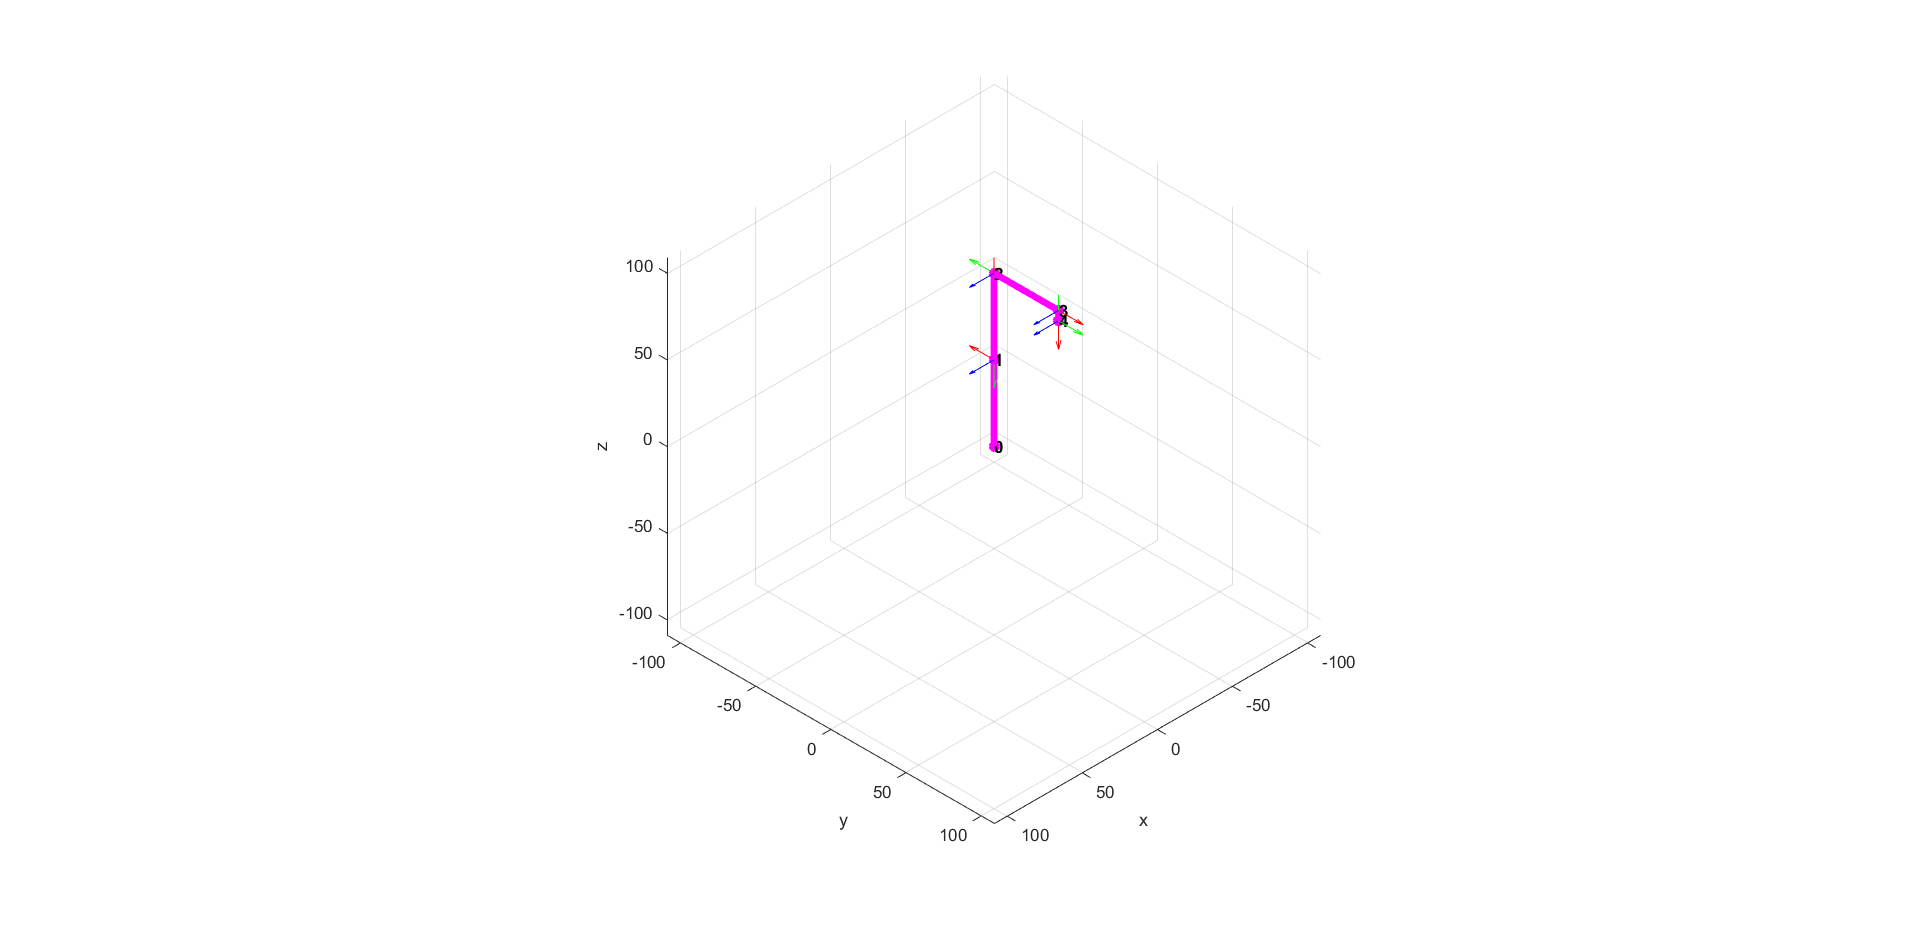
\includegraphics[width=1\textwidth]{img/robotFinal_DH.png}
    \caption{Prueba DH Robot}
    \label{fig:pruebaDH_robot}
\end{figure}
El dibujo creado concuerda con el diagrama de Denavit Hartenberg y con el modelo 3D del robot en Solidworks, por lo tanto se definieron los parametros y características correctamente.

\section{Cinemática Diferencial}
Las siguientes gráficas representan el cambio de posición, velocidad y aceleración del efector final respecto al tiempo. En la parte superior, la posición muestra la trayectoria en los ejes X, Y y Z; como se puede observar, se presenta una trayectoria de tipo sinusoidal o cosenoidal. En la gráfica de la velocidad lineal, las curvas indican cambios bruscos de dirección, aceleraciones y desaceleraciones a lo largo del tiempo. Por último, la aceleración indica variaciones rápidas de velocidad, es decir, aceleraciones intensas.

En la segunda parte, se muestra la orientación del efector final en coordenadas de Euler, donde $\phi$ representa la rotación en X, $\theta$ rotación en Y, y $\theta$ rotación en Z. La velocidad angular presenta la rapidez de cambio de los ángulos y la aceleración indica los cambios en la velocidad angular, útil para estimar esfuerzos dinámicos. 

\begin{figure}[H]
    \centering
    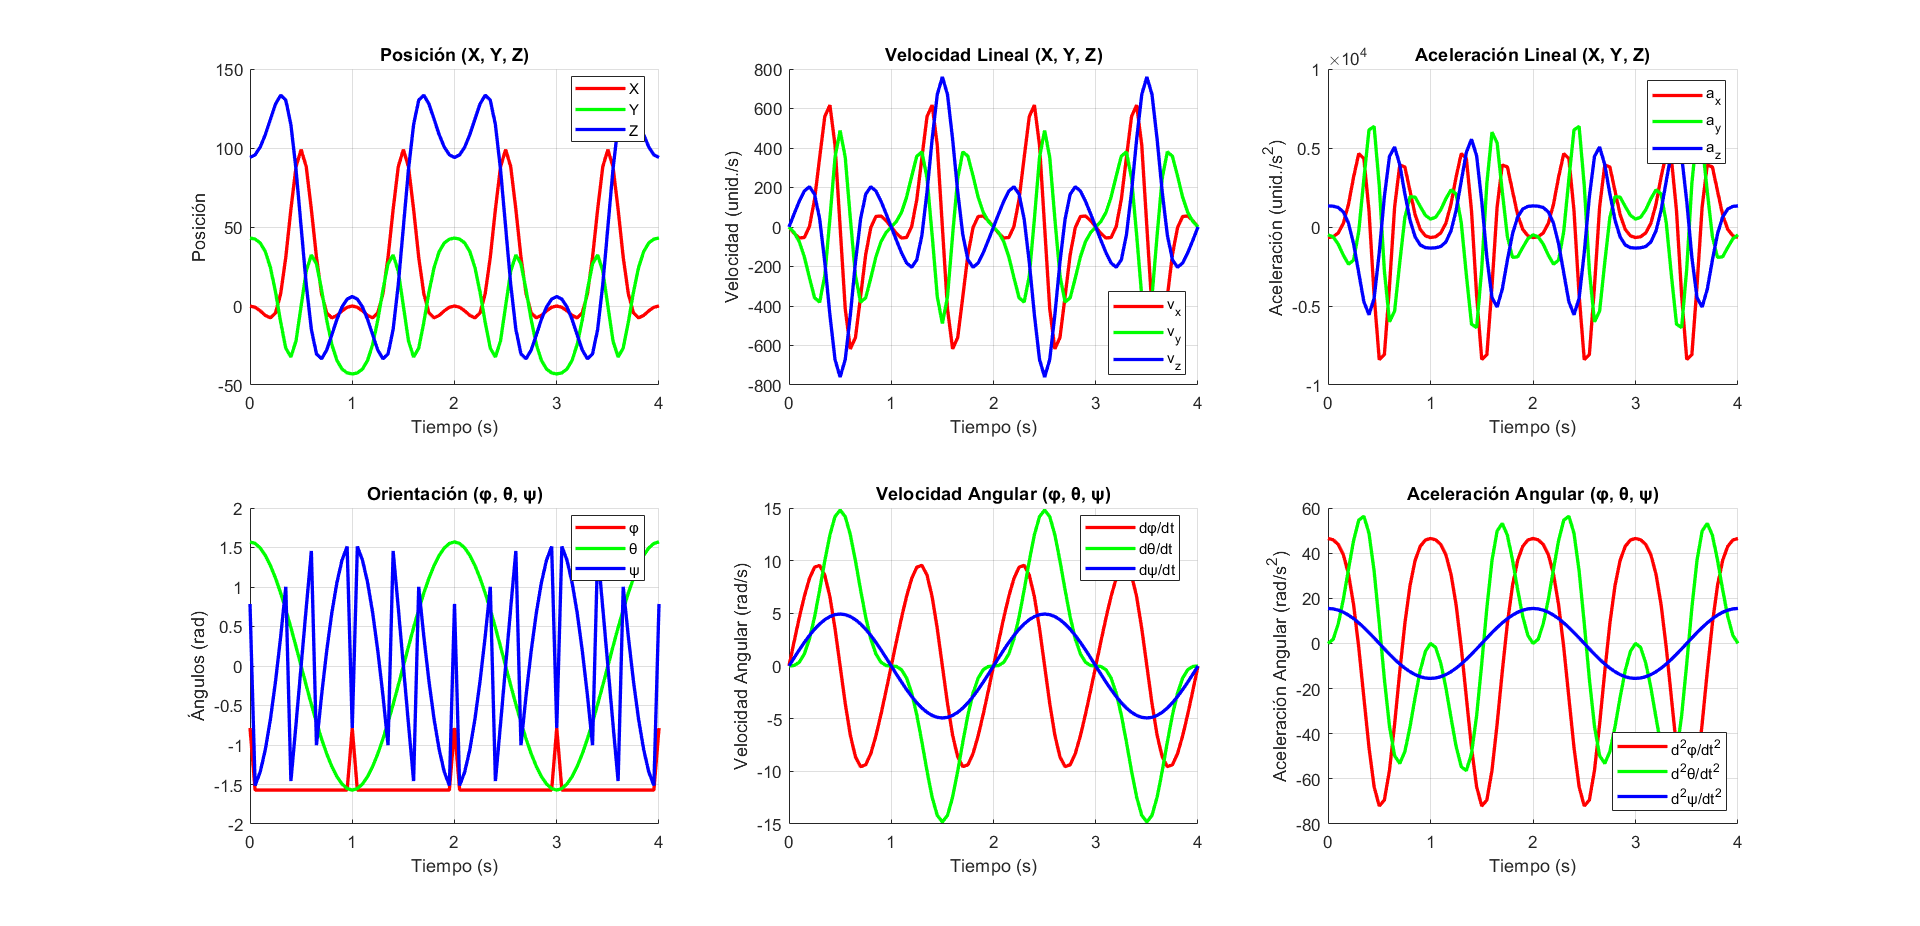
\includegraphics[width=1\textwidth]{img/graficas_diferencial.png}
    \caption{Gráficas Cinemática Diferencial}
    \label{fig:grafica_diferencial}
\end{figure}

\pagebreak

\section{Cinemática Inversa}

Para la primera prueba, se utilizó una trayectoria sencilla, la cual consiste en una rotación del eje Z, manteniendo constante la posición cartesiana. La trayectoria se muestra en la siguiente tabla. 
\begin{table}[H]
    \centering
    \begin{tabular}{|c|c|c|c|}
    \hline
    \textbf{x} & \textbf{y} & \textbf{z} & \textbf{Periodo (s)} \\
    \hline
    -50 & 50  & 50 & 0 \\
    50  & -50 & 50 & 2 \\
    \hline
    \end{tabular}
    \caption{Puntos de la trayectoria cartesiana}
    \label{tab:trayectoria}
\end{table}

Los dos puntos fueron alcanzados exitosamente, ya que el error de posición esta dentro del rango de tolerancia previamente definido. 
\begin{itemize}
    \item Solución alcanzada en muestra 3, iteraciones 18, error = 9.806690e-04
    \item Solución alcanzada en muestra 1, iteraciones 17, error = 5.572133e-04
\end{itemize}
La siguiente figura muestra la postura final del robot en el espacio 3D.

\begin{figure}[H]
    \centering
    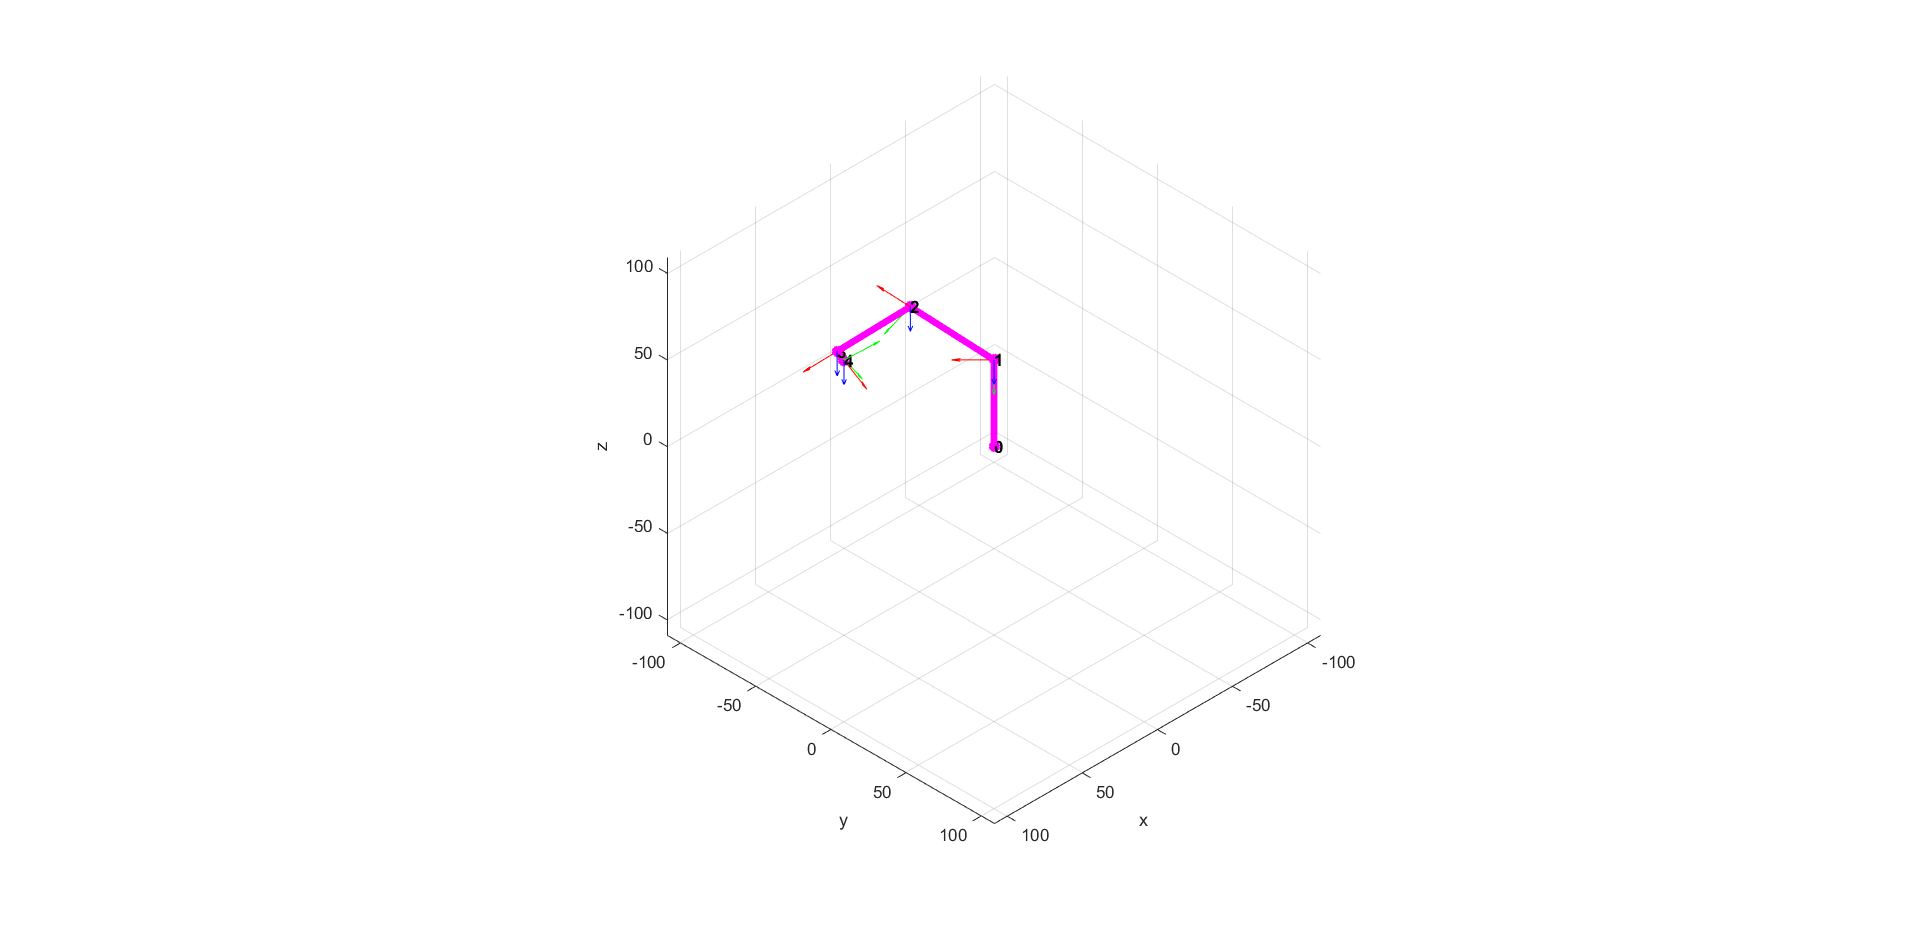
\includegraphics[width=1\textwidth]{img/diagrama_inversa.png}
    \caption{Animación Cinemática Inversa Ejemplo 1}
    \label{fig:diagrama_inversa1}
\end{figure}

Como se puede observar en la figura \autoref{fig:grafica_inversa1} la posición en Z permanece constante, mientras X y Y no. Esto representa el movimiento de rotación en el eje Z. La orientación, expresada en ángulos de Euler ($\phi$, $\theta$, $\psi$), muestra un cambio evidente. El valor de $\psi$ (azul) varía aproximadamente 40°, reflejando una rotación sobre el eje Z del efector.

La velocidad y aceleración angular muestran actividad pronunciada en las tres componentes, lo cual sugiere que la orientación fue modificada no solo en Z, sino compensada también por pequeños ajustes en $\phi$ y $\theta$.

\begin{figure}[H]
    \centering
    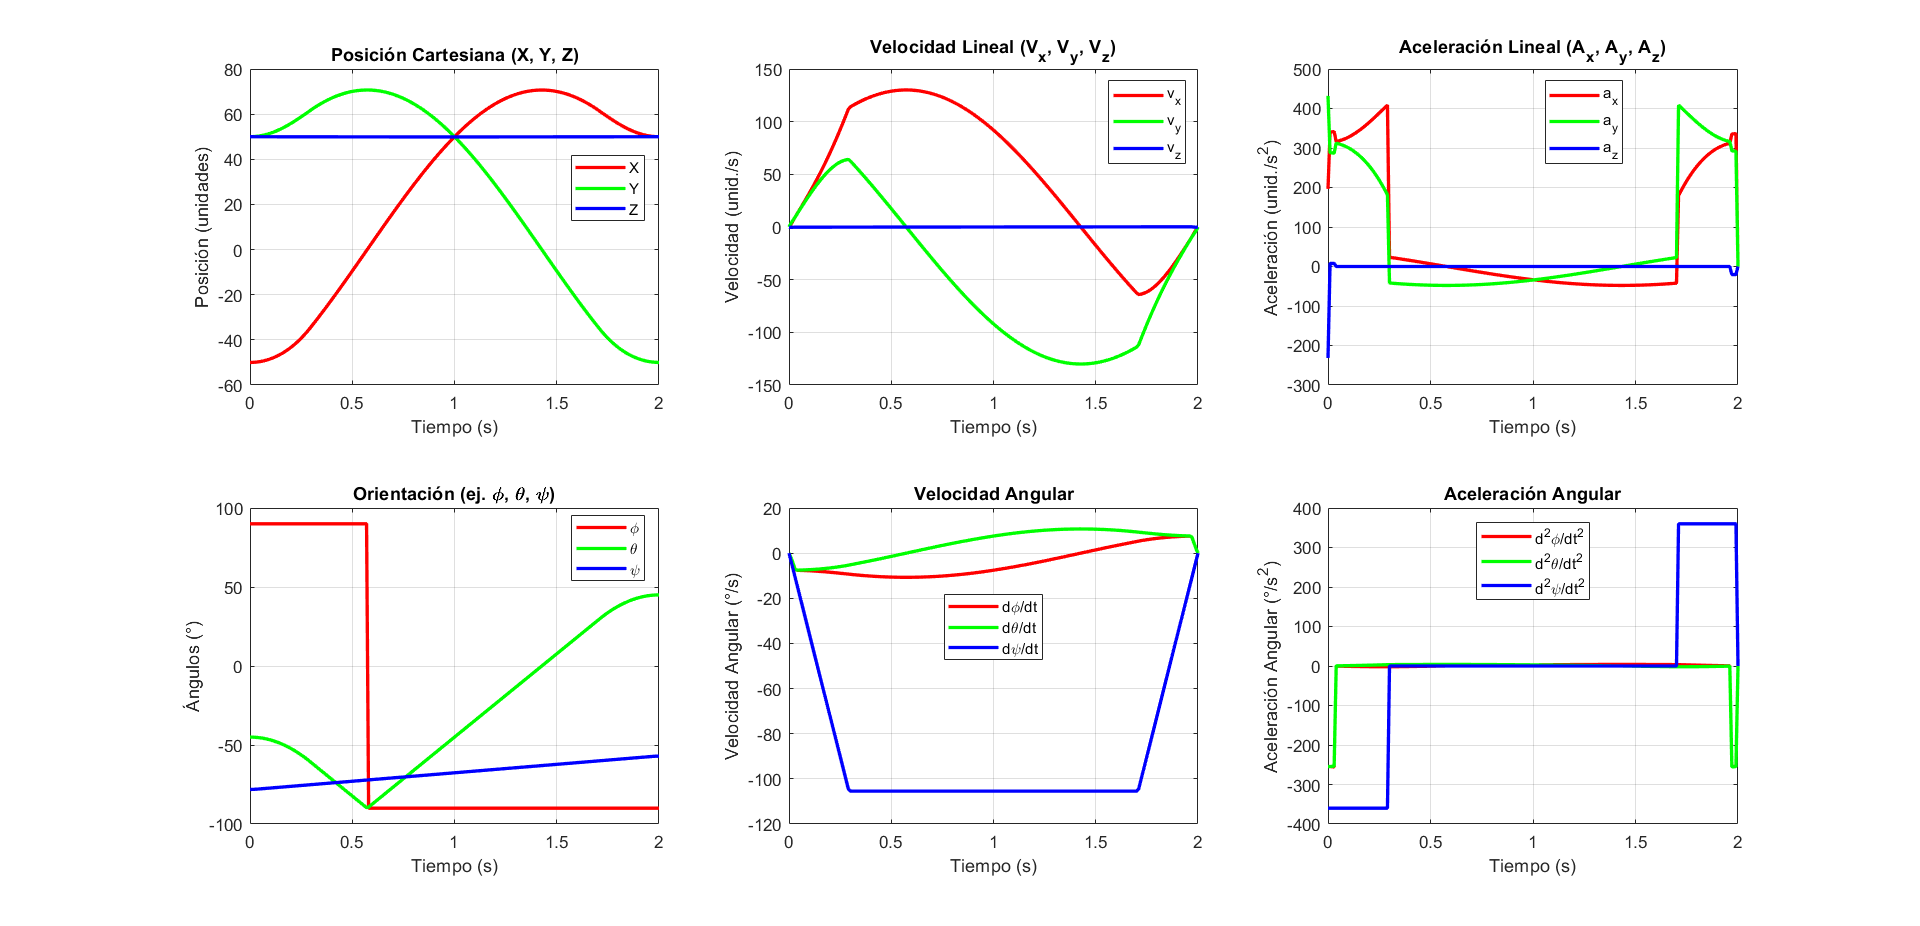
\includegraphics[width=1\textwidth]{img/graficas_inversa.png}
    \caption{Gráficas Cinemática Inversa Ejemplo 1}
    \label{fig:grafica_inversa1}
\end{figure}

La \autoref{fig:cinematica_articular1} muestra la evolución de los ángulos articulares, velocidades y aceleraciones a lo largo del tiempo. La articulación 1 presenta un cambio significativo desde aproximadamente 135° hasta -45°, lo cual significa una rotación de 180° de la base del robot.

Las articulaciones 2,3 y 4 mantienen valores casi constantes con leves ajustes, necesarios para conservar la orientación deseada del efector. Las gráficas de velocidad y aceleración de la articulación 1 presentan un perfil trapezoidal, típico de un movimiento planificado con trayectoria tipo “trapecio”, lo cual indica una transición suave y controlada.

\begin{figure}[H]
    \centering
    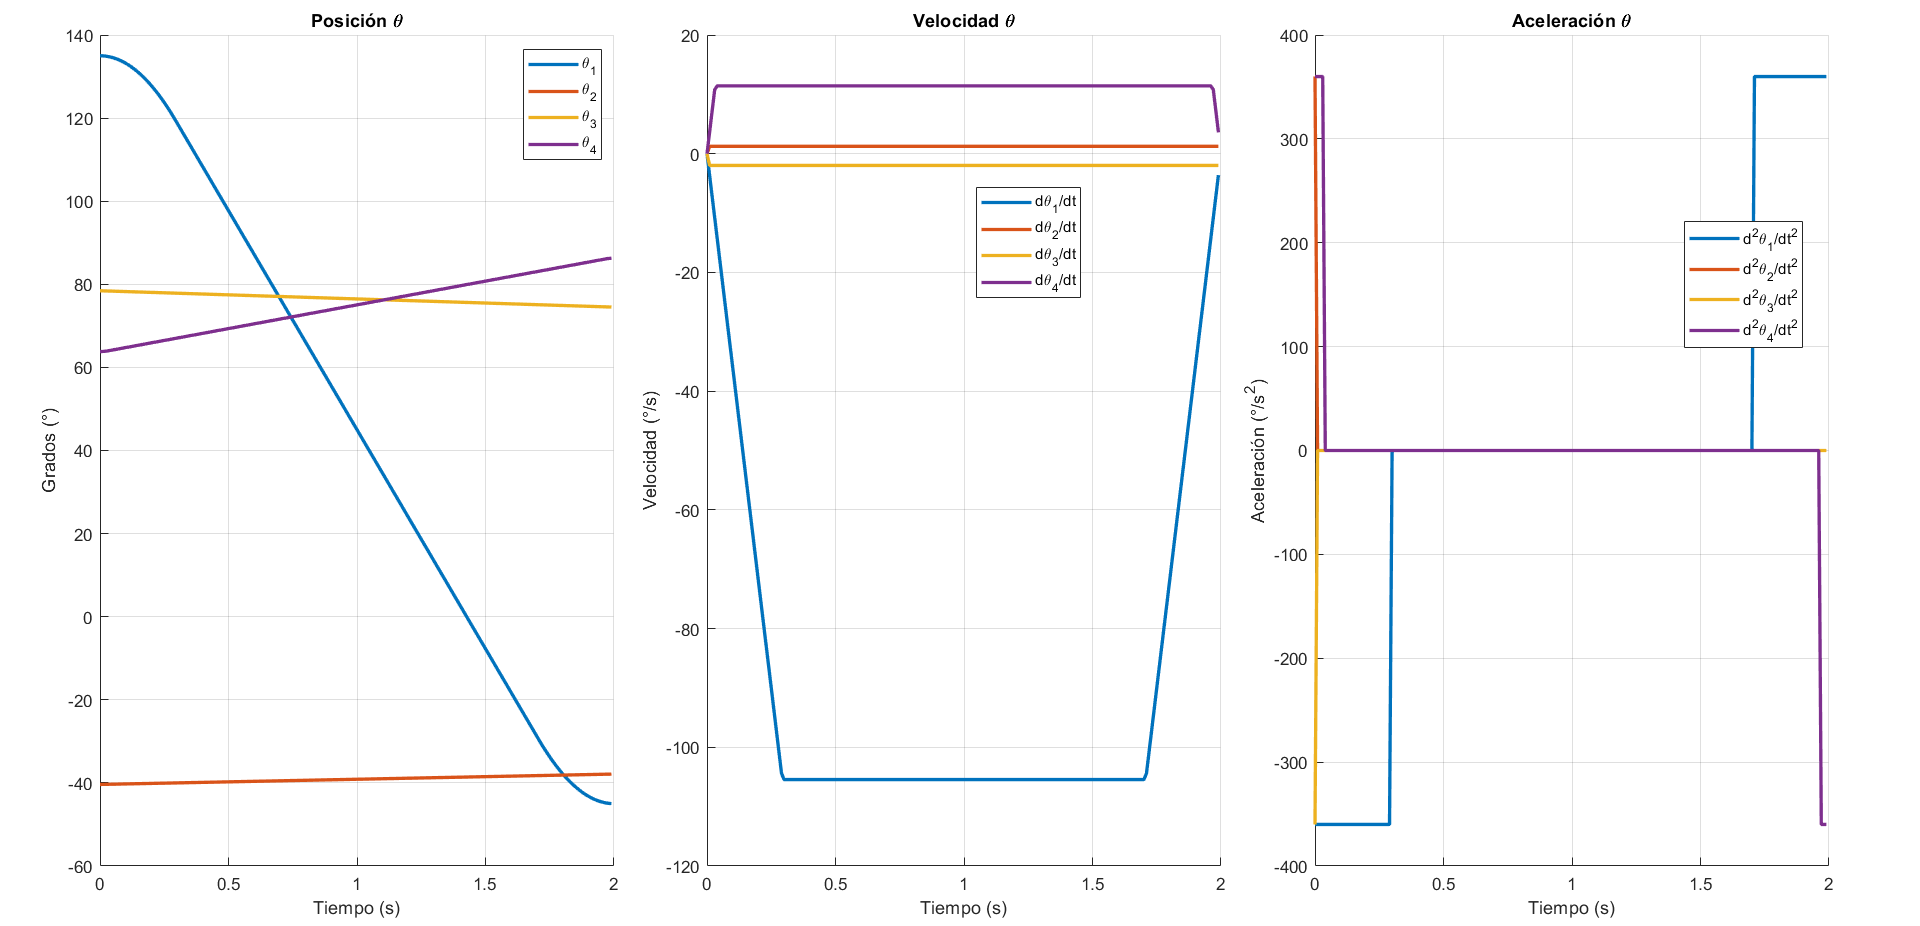
\includegraphics[width=1\textwidth]{img/cinematica_articular.png}
    \caption{Gráficas Cinemática Articular Ejemplo 1}
    \label{fig:cinematica_articular1}
\end{figure}

\pagebreak

Además del primer caso de prueba, se realizó un segundo experimento en el cual se diseñó una trayectoria \textbf{más compleja compuesta por tres puntos cartesianos}. Esta nueva trayectoria fue elegida de forma que:

\begin{itemize}
    \item Requiriera movimiento en las cuatro articulaciones del robot.
    \item Incluyera una rotación significativa de la base (articulación $\theta_1$).
    \item Combinara desplazamientos en el espacio con cambios en la orientación del efector.
\end{itemize}

La ejecución de esta trayectoria permitió validar la capacidad del algoritmo de cinemática inversa para resolver configuraciones más desafiantes, logrando convergencia en todos los puntos con errores menores al umbral especificado. Las gráficas resultantes mostraron perfiles dinámicos en todas las variables articulares y espaciales, evidenciando una correcta coordinación entre posición y orientación del efector.

\begin{itemize}
    \item Solución alcanzada en muestra 2, iteraciones 19, error = 5.010011e-04
    \item Solución alcanzada en muestra 1, iteraciones 17, error = 6.168571e-04
    \item Solución alcanzada en muestra 1, iteraciones 17, error = 6.168571e-04
\end{itemize}


\begin{figure}[H]
    \centering
    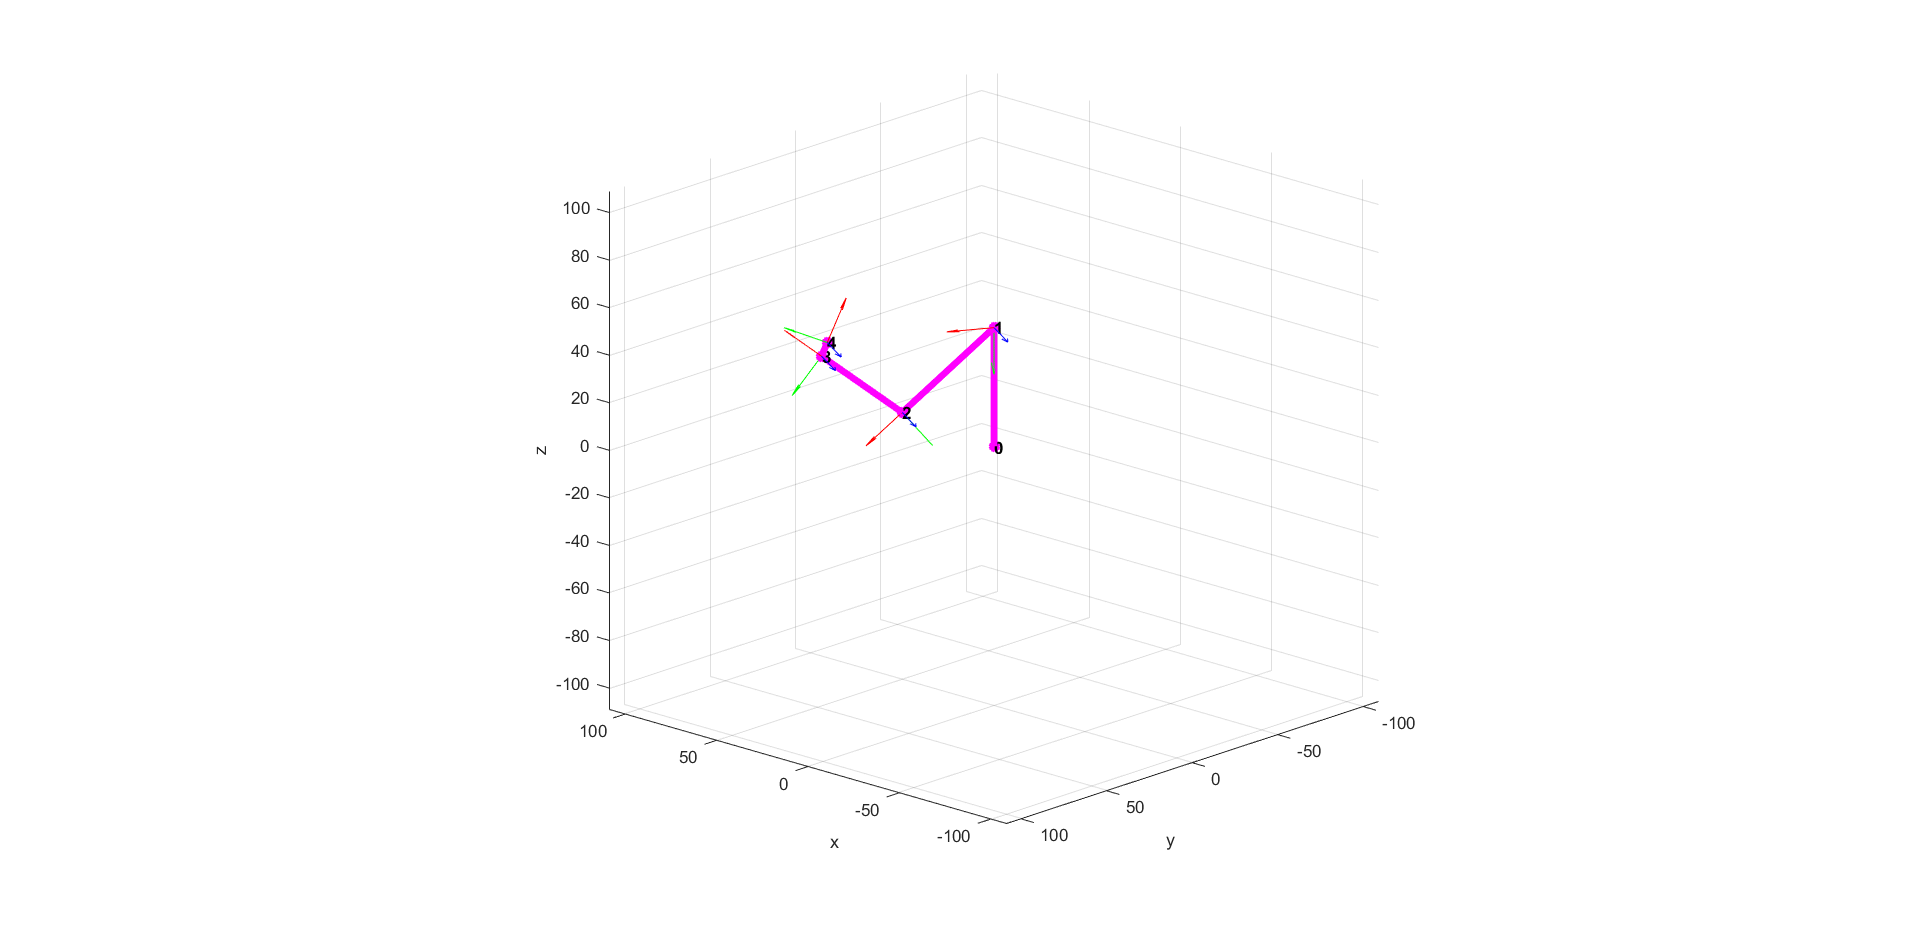
\includegraphics[width=1\textwidth]{img/animacion_inversa2.png}
    \caption{Animación Cinemática Inversa 2}
    \label{fig:diagrama_inversa1}
\end{figure}

\begin{figure}[H]
    \centering
    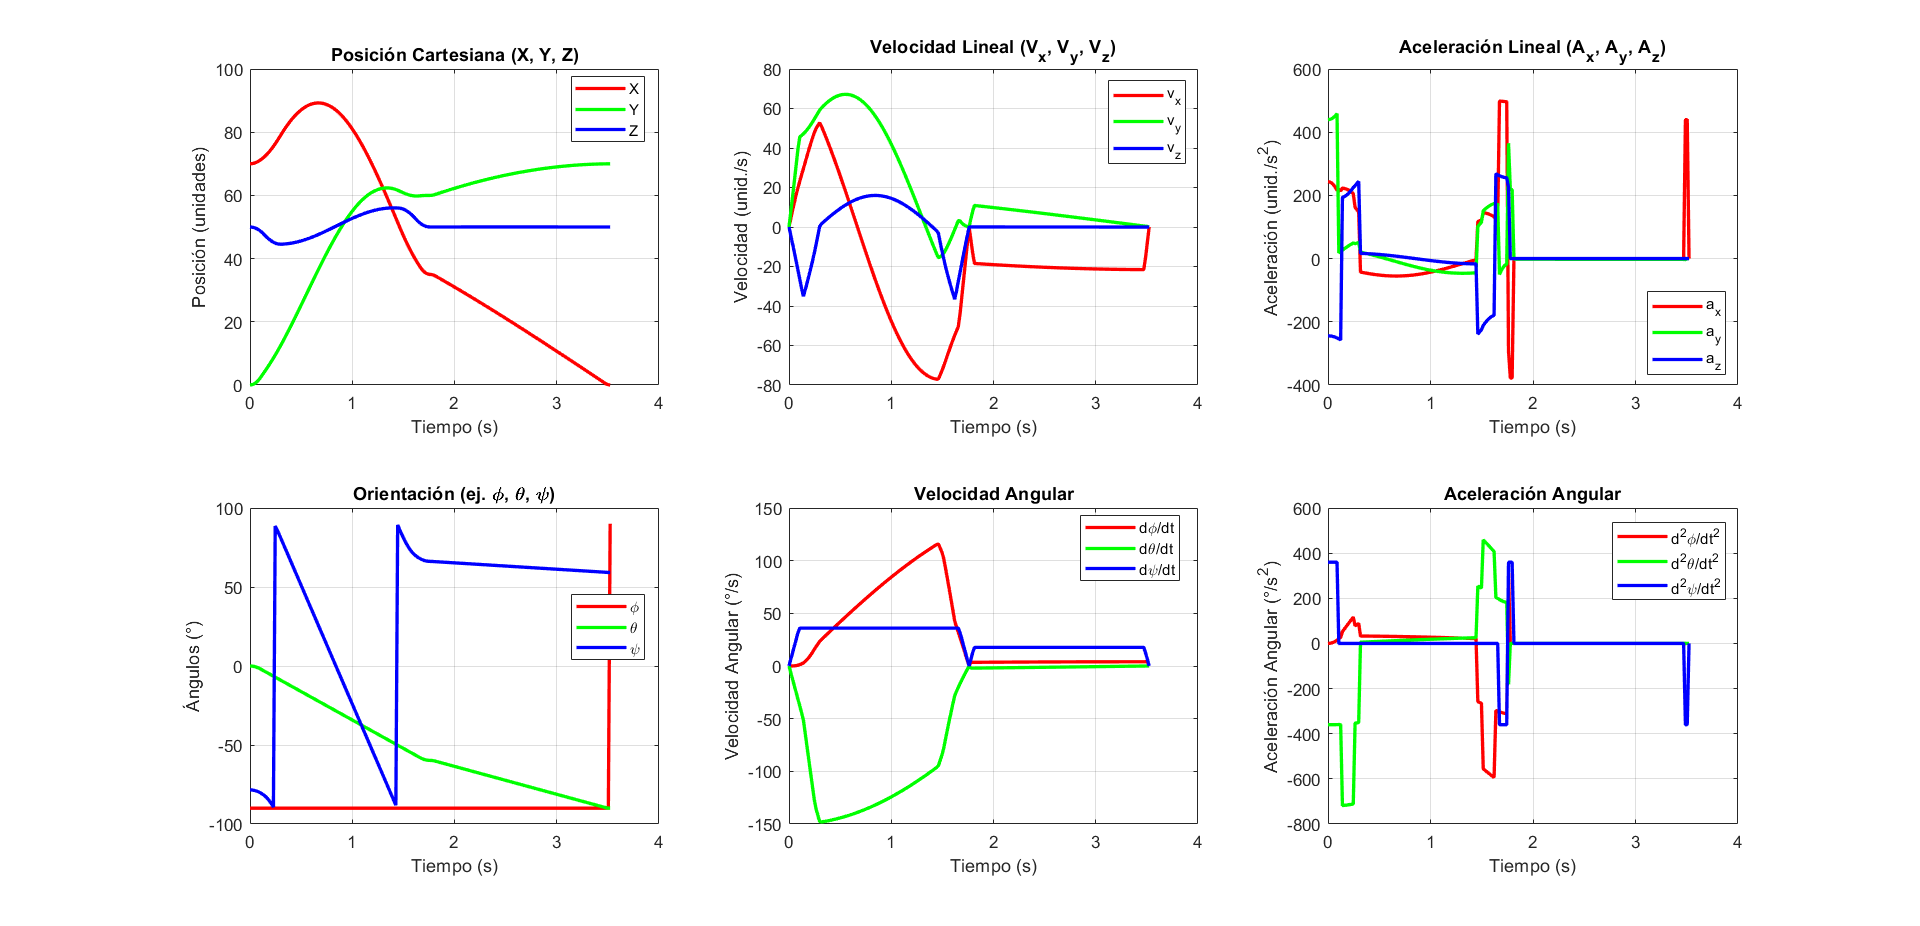
\includegraphics[width=1\textwidth]{img/graficas_inversa2.png}
    \caption{Gráficas Cinemática Inversa Ejemplo 2}
    \label{fig:grafica_inversa1}
\end{figure}

\begin{figure}[H]
    \centering
    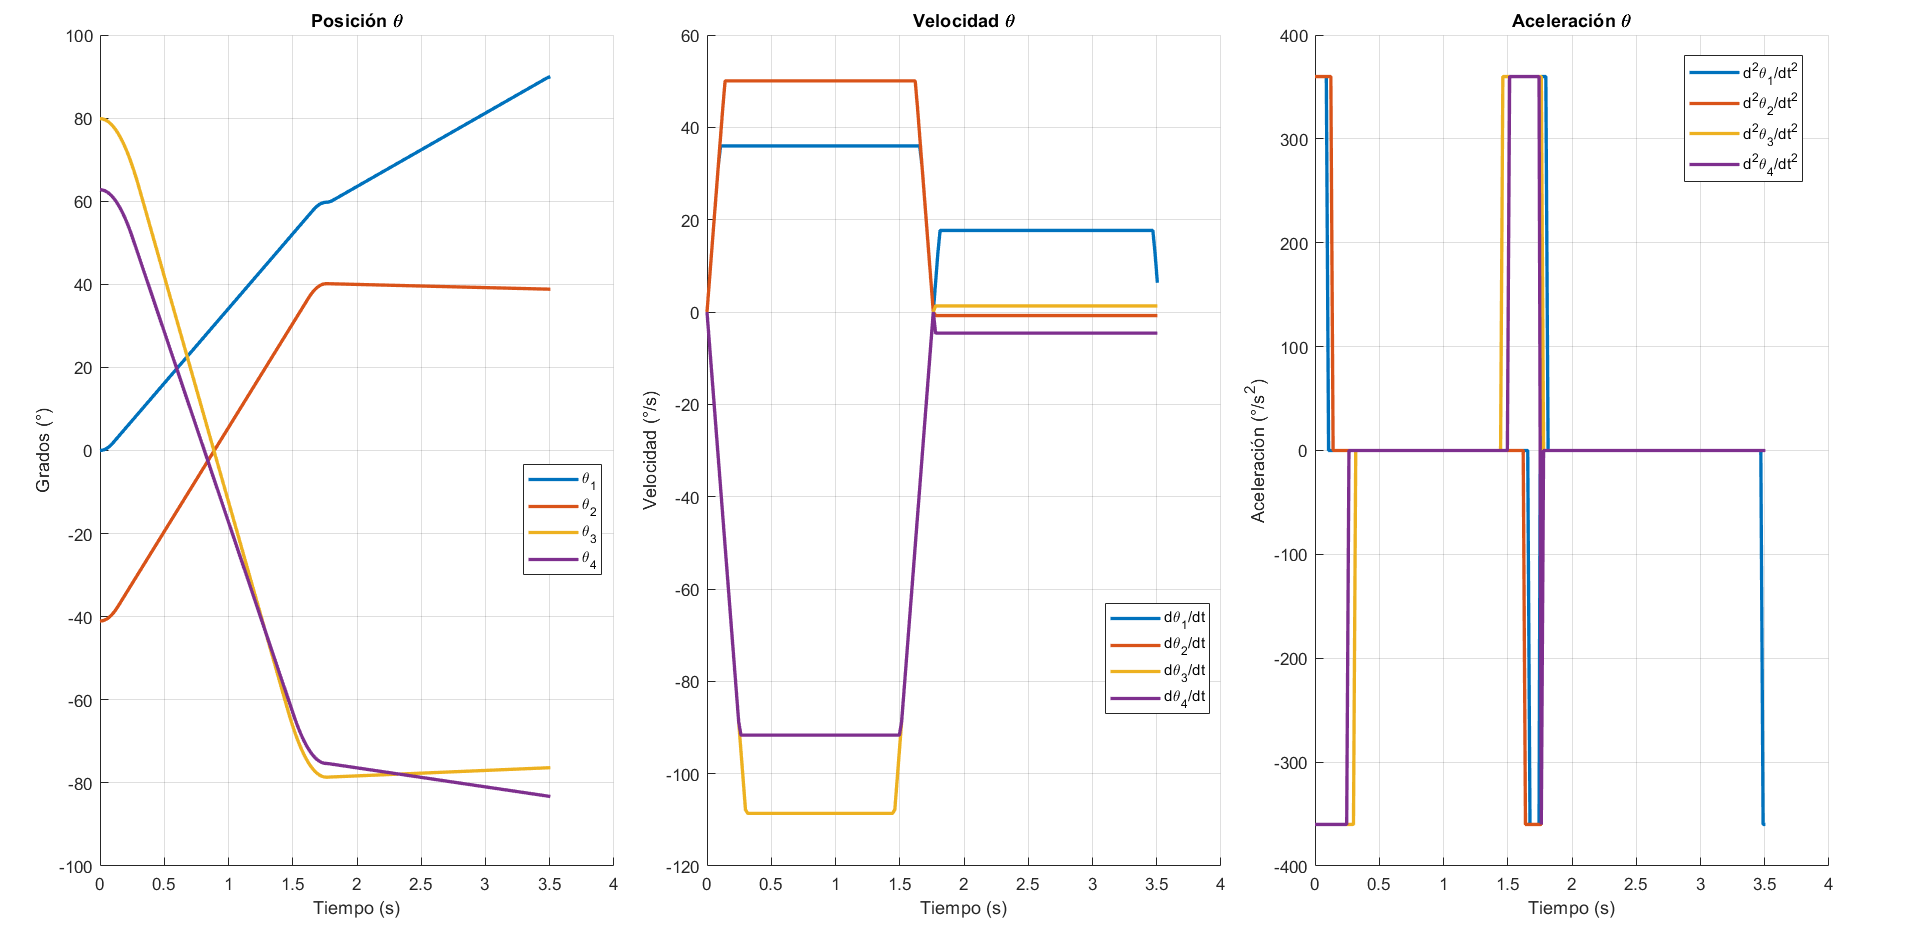
\includegraphics[width=1\textwidth]{img/cinematica_articular2.png}
    \caption{Gráficas Cinemática Articular Ejemplo 2}
    \label{fig:cinematica_articular2}
\end{figure}